\section{Rechnermodell}
\label{sec:rechnermodell}

\textbf{Rechnermodell -- von-Neumann-Rechner}
\begin{figure}[ht]
  \centering
  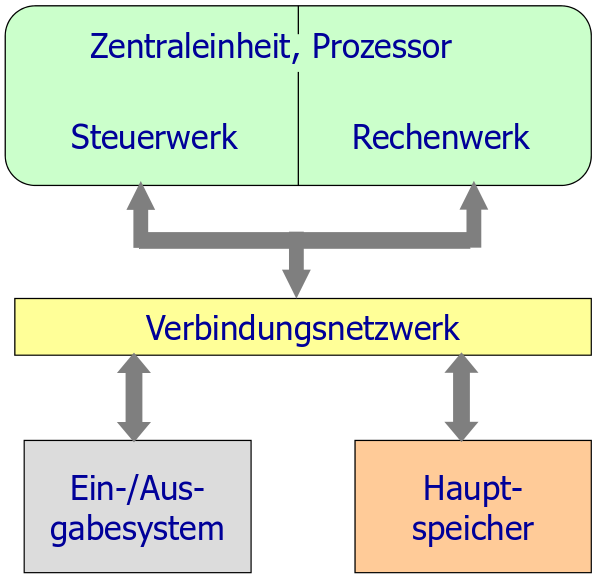
\includegraphics[width=0.33\textwidth]{VonNeumann}
  \label{VonNeumann}
\end{figure}

\textbf{Von-Neumann-Rechner -- Komponenten}
\begin{items}
	\item \underline{Zentraleinheit}: Verarbeitet Daten gemäß eines Programms
	\begin{enumeration}
		\item \textbf{Leitwerk/Steuerwerk}: Holt Programmbefehle aus Speicher, entschlüsselt sie, steuert Ausführung
		\item \textbf{Rechenwerk/ALU}: Führt arithmetische/logische Operationen aus, wird beeinflussst durch Steuersignale, liefert Meldesignale an Steuerwerk
	\end{enumeration}
	\item \underline{Hauptspeicher}: Besteht aus eindeutig adressierbaren Speicherzellen, bewahrt Programme \emph{und} Daten auf (im Gegensatz zur \emph{Harvard-Architektur})
	\item \underline{Bussystem}:
	\begin{enumeration}
		\item \textbf{Adressleitungen}: Transportieren unidirektional Adressinformationen
		\item \textbf{Datenleitungen}: Transportieren bidirektional Daten und Befehle (von/zum Prozessor)
		\item \textbf{Steuerleitungen}: Transportieren uni- oder bidirektional Steuerinformationen (von/zum Prozessor)
	\end{enumeration}
	\item \underline{Ein-/Ausgabesystem}: Geräte zur Eingabe von Daten/Programmen bzw. zur Ausgabe von Daten (angebunden durch Bussysteme)
\end{items}

\newpage

\textbf{Rechnermodell -- einfacher Mikroprozessor}
\begin{figure}[ht]
  \centering
  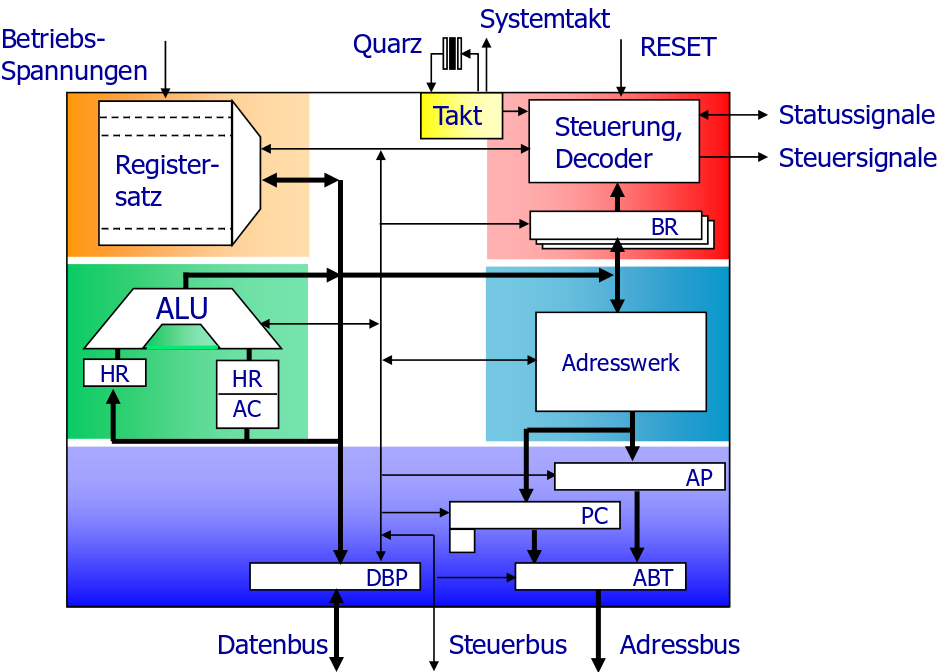
\includegraphics[width=0.33\textwidth]{Mikroprozessor}
  \label{Mikroprozessor}
\end{figure}
\begin{items}
	\item \underline{\textcolor{red!90!black}{Steuerwerk}}: Steuert die Systemkomponenten (meist \emph{dynamisches Schaltwerk} $\leadsto$ Zustandsinformation in Kondensatoren gespeichert $\leadsto$ Refresh-Taktfrequenz erforderlich, sonst Informationsverlust)
	\begin{enumeration}
		\item \textbf{Befehlsregister}: enthält den gerade ausgeführten Befehl (besteht aus mehreren Registern: unterschiedlich lange Befehlsformate bzw. Vorabladen von Befehlen)
		\item \textbf{Decoder}: dekodiert Befehlsworte (= mikroprogrammiertes/festverdrahtetes Schaltwerk)
		\item \textbf{Taktgenerator}: erzeugt Systemtakt (durch externen Quarz), erzeugt ein mit Prozessortakt synchronisiertes Rücksetzsignal (startet Initialisierungsroutine des Steuerwerks)
		\item \textbf{Steuerregister}: Ermöglicht Beeinflussung der aktuellen Arbeitsweise des Steuerwerks (Interrupt enable Bit: wird auf Unterbrechungsanforderung am \code{INT}-Eingang reagiert?, User/System Bit: Sind alle Befehle nutzbar oder nur bestimmte?, Trace Bit: Unterbrechungsroutine nach jeder Befehlsausführung starten?, Decimal Bit: Dual oder BCD rechnen?)
	\end{enumeration}
	\item Befehlsausführung:
	\begin{enumeration}
		\item Holphase: nächster Befehl wird in Befehlsregister geladen
		\item Dekodierphase: Decoder ermittelt Startadresse des Mikroprogramms, welches Befehl ausführt
		\item Ausführungsphase: Mikroprogramm führt Befehl aus, indem Signalfolgen an andere Komponenten übermittelt und Meldesignale ausgewertet werden
	\end{enumeration}

	\item \underline{\textcolor{green!60!black}{Rechenwerk}}: Führt vom Steuerwerk verlangte logische/arithmetische Operationen aus (reines Schaltnetz)
	\begin{enumeration}
		\item \textbf{Statusregister}: informiert Steuerwerk über Ablauf des Ergebnisses (Übertrag \code{CF}, Hilfsübertrag \code{AF}, Null \code{ZF}, Vorzeichen \code{SF}, Überlauf \code{OF}, Even \code{EF}, Parität \code{PF})
		\item \textbf{Hilfsregister/Akkumulatoren}: Zwischenspeichern von Operanden und Ergebnissen (meist zweigeteilt: Akkumulator-Register \code{AC} + nachgeschaltetes Hilfsregister \code{HR} (Latch))
		\item \textbf{Busse}: 2 Eingangsbusse (Operanden), 1 Ausgangsbus (Ergebnis)
		\item \textbf{Ergebnisse}: Werden entweder in Prozessor-Registern gespeichert, zu ALU-Eingangsregistern zurückgeführt oder über externen Datenbus an andere Systemkomponenten übergeben
	\end{enumeration}
	\item Varianten:
	\begin{enumeration}
		\item \textbf{Variante A}: Hilfsregister des Akkumulators hinter der ALU (Vorteil: ALU-Operationen ohne Akkumulatorveränderung möglich. Nur bei alten 8 Bit-Prozessoren)
		\item \textbf{Variante B}: Rechenwerk ohne Akkumulator - Akkumulator in Prozessor-Registersatz verlegt (Vorteil: Mehrere Register können Akkumulatorfunktionen übernehmen. Bei allen modernen 16/32 Bit-Prozessoren)
	\end{enumeration}

	\newpage

	\item Operationen:
	\begin{enumeration}
		\item Arithmetische Operationen (Addieren/Subtrahieren ohne/mit Übertrag, Inkrementieren/Dekrementieren, Multiplizieren/Dividieren ohne/mit Vorzeichen, Komplement)
		\item Logische Verknüpfungen (Negation, Und, Oder, Antivalenz)
		\item Schiebe-/Rotationsoperationen (Links-/Rechts-Verschieben, Links/Rechts ohne/mit Übetragsbit rotieren)
		\item Transportoperationen (Transferieren: move, load, store,\dots)
	\end{enumeration}

	\item \underline{\textcolor{orange}{Registersatz}}: Zwischenspeicherung von häufig benutzten Operanden $\leadsto$ schnellerer Zugriff als auf Hauptspeicher
\end{items}